\documentclass[a4paper, 12 pt]{article}

\usepackage{graphicx}
\usepackage{bm}

\author{Guillaume Tollini}

\title{TVC Rocket dynamics}

\date{\vfill \today}

\begin{document}

\maketitle

\newpage

\section*{Objective}
\addcontentsline{toc}{section}{\protect\numberline{}Objective}
This document explains the steps I followed in order to choose and code my rocket dynamic model

\newpage

\section*{IMPORTANT}
\addcontentsline{toc}{section}{\protect\numberline{}IMPORTANT}
This model is wrong. The formula for torque is inexact. Further modifications will come soon


\newpage

\tableofcontents

\newpage


\section{Mathematical model}
\subsection{Reference frames}
\begin{figure}[!h]
\hspace{0 cm}
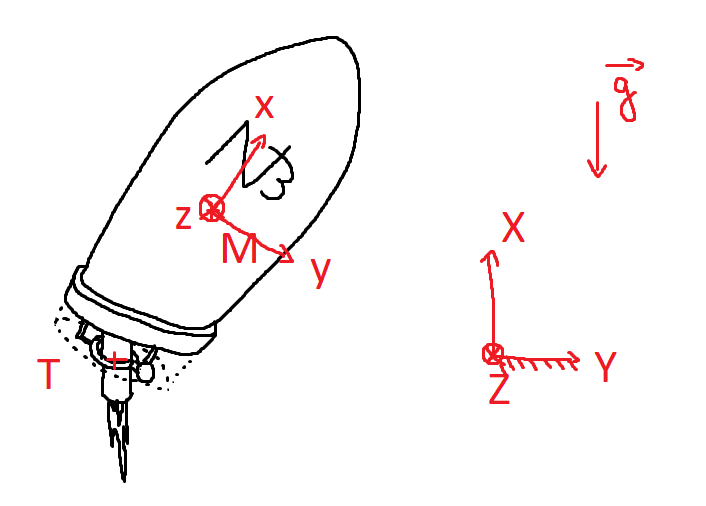
\includegraphics[width=0.9\textwidth]{schema-fusee.png}
\caption{Reference frames}
\end{figure}

$\mathcal{R}_{Earth}$ is the inertial reference frame that is fixed to Earth, it is associated with the vector basis $\bm x\bm y\bm z$. $\mathcal{R}_{AUV}$ is the reference frame that is fixed to the AUV. It is not inertial and associated with the vector basis $\bm X\bm Y\bm Z$.

\begin{figure}[!h]
\begin{tabular}{| l l c c c |}
\hline
\parbox[t]{2.8 cm}{Degree of\newline freedom (DOF)}	& Description	& \parbox[t]{1.6 cm}{Force or \newline moment}	& Velocity	& \parbox[t]{2.3 cm}{Position and \newline Euler angles} \\
\hline \hline
1			& surge direction (x-axis)			& $X$	& u		& $x$ \\
2			& sway direction (y-axis)			& $Y$	& v		& $y$ \\
3			& heave direction (z-axis)			& $Z$	& w		& $z$ \\
4			& roll : rotation about the (x-axis)		& $K$	& p		& $\phi$ \\
5			& pitch : rotation about the (y-axis)		& $M$	& q		& $\theta$ \\
6			& yaw : rotation about the (z-axis)		& $N$	& r		& $\psi$ \\
\hline
\end{tabular}
\caption{Main variables of movement}
\label{variables}
\end{figure}

\subsection{Definition of vectors of interest}
In this document, all vectors and matrices will appear in bold. Vectors defined here after will be used in the mathematical model of tue AUV :

$$\bm\eta = \left[ 
\begin{array}{c}
\bm{\eta}_1	\\
\bm{\eta}_2
\end{array}
\right], \; \bm{\eta}_1 = \left[ 
\begin{array}{c}
x	\\
y	\\
z
\end{array}
\right], \; 
{\bm\eta}_2 = \left[ 
\begin{array}{c}
\phi	\\
\theta	\\
\psi
\end{array}
\right]$$

$$\bm\nu = \left[ 
\begin{array}{c}
\bm{\nu}_1	\\
\bm{\nu}_2
\end{array}
\right], \; \bm{\nu}_1 = \left[ 
\begin{array}{c}
u	\\
v	\\
w
\end{array}
\right], \; 
{\bm\nu}_2 = \left[ 
\begin{array}{c}
p	\\
q	\\
r
\end{array}
\right]$$

$$\bm\tau = \left[ 
\begin{array}{c}
\bm{\tau}_1	\\
\bm{\tau}_2
\end{array}
\right], \; \bm{\tau}_1 = \left[ 
\begin{array}{c}
X	\\
Y	\\
Z
\end{array}
\right], \; 
{\bm\tau}_2 = \left[ 
\begin{array}{c}
K	\\
M	\\
N
\end{array}
\right]$$

\section{Equations of movement}

Newton's law gives :

$$m\dot{\bm \nu}_1} = {\bm\tau}_1 + \vec{\bm F}_i + \vec{\bm F}_C$$ where ${\bm\tau}_1$ is the sum of forces, $\vec{\bm F}_i$ is the inertia fictitious force and $\vec{\bm F}_C$ the Coriolis fictitious force.

which rewrites :


$$m({\dot\bm\nu_1} + {\dot\bm{\nu}_2} \times\bm\nu_1) = {\bm\tau}_1$$

and :

$${\dot\bm\nu_1} = \frac{{\bm\tau}_1}{m} - {\bm{\nu}_2}\times\bm\nu_1$$

Thus in the body-fixed reference frame we have :

$$\left[
\begin{array}{c}
\dot \bm u\\
\dot \bm v\\
\dot \bm w
\end{array}
\right] =
\left[
\begin{array}{c}
\frac{X}{m} - (qw - rv)\\
\frac{Y}{m} - (ru - pw)\\
\frac{Z}{m} - (pv - qu)
\end{array}
\right]$$

And for the torques, using the inertia matrix relative to the center of mass $\bm I_G$, we have :

$$\bm I_G {\dot\bm\nu_2} + {\bm\nu}_2\times\bm I_G \bm{\nu}_2) = {\bm\tau}_2$$

with :

$$\bm I_G =
\left[
\begin{array}{c c c}
I_{x} & I_{xy} & I_{xz} \\
I_{xy} & I_{y} & I_{yz} \\
I_{xz} & I_{yz} & I_{z}
\end{array}\right]$$

With only $I_{xx}$, $I_{yy}$ and $I_{zz}$ not null.

Thus in the body-fixed reference frame we have :

$$\left[
\begin{array}{c}
\dot \bm p\\
\dot \bm q\\
\dot \bm r
\end{array}
\right] =
\left[
\begin{array}{c}
\frac{K}{I_x} - qr(I_z-I_y)\\
\frac{M}{I_y} - rp(I_x - I_z)\\
\frac{N}{I_z} - pq(I_y - I_x)
\end{array}
\right]$$

\section{Forces}

The vector $\bm \tau$ of forces and moments can be decomposed into several vectors, each regrouping the actions of different physical origins :

\begin{itemize}
\item $\bm {\tau}_G$ for the action of gravity
\item $\bm {\tau}_D$ for the drag due to the surrounding air
\item $\bm {\tau}_C$ for the actions influenced by the control inputs
\end{itemize}

\subsubsection{Weight}

$\bm W$ is the weight vector of the rocket.
Then $\bm W_{\mathcal{B}} = \bm W|{\bm x\bm y\bm z} = [0 \; 0 \; -mg]^T$ ($\bm z$ is upwards).
Since $\bm W|{\bm x\bm y\bm z} = \bm J_1\cdot \bm W|_{\mathcal{B}}$, 
and because $\bm J_1$ is orthogonal we have $\bm W|_{\mathcal{B}} = \bm J_1^{T}\cdot [0 \; 0 \; -mg]^T$.

The weight gives no angular momentum.

\subsection{Drag}

Let us say for now that these are negligible.

\subsection{Thrust vector control}

Let us call $T$ the norm of the thrust vector (which is the action of thrust on the rocket). We rotate the rocket-fixed reference frame $\bm{XYZ}$ of an angle $\alpha_1$ about $\bm x$ and
name the new reference frame $\bm{x'yz'}$. We then rotate this reference frame of an angle $\alpha_2$ about $\bm y'$ and we get the reference frame
$\bm{X'Y'Z''}$. $\bm Z''$ is the vector carrying th thrust vector. $\alpha_1$ and $\alpha_2$ are the two command angles.

We have :

$$\bm{\tau}_C = -T \bm Z'' = \bm R_Z(\alpha_2) \cdot \bm R_Y(\alpha_1) \cdot \left[\begin{array}{c} 0 \\ 0 \\ Y \end{array}\right]$$



\end{document}
